\begin{frame}
\frametitle{Объектно Центричный Визуальный Контроль}

\begin{columns}[t]
\begin{column}{0.43\linewidth}
    Обычная задача визуального контроля включает в себя:
    \begin{itemize}
        \item Актуатор, напрямую контролируемый действиями
        \item Объекты, косвенно контролируемые актуатором
        \item Функцию награды, подразумевающую взаимодействие между актуатором и объектом(-ами).
    \end{itemize}
\end{column}

\begin{column}{0.55\linewidth}
    \begin{figure}
    \centering
    \begin{subfigure}[c]{.45\linewidth}
        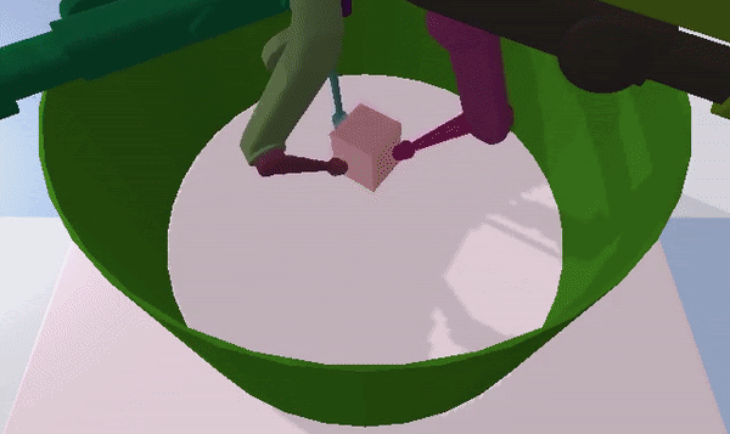
\includegraphics[width=\linewidth]{images/visual_control_envs/causal_world.png}
    \end{subfigure}
    \hspace{1em}
    \begin{subfigure}[c]{.45\linewidth}
        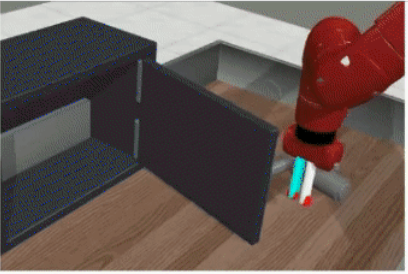
\includegraphics[width=\linewidth]{images/visual_control_envs/metaworld.png}
    \end{subfigure}
    \vspace{3em}
    
    \begin{subfigure}[c]{.45\linewidth}
        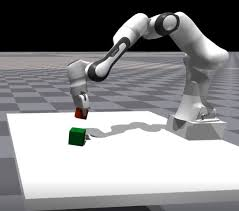
\includegraphics[width=\linewidth]{images/visual_control_envs/isaac_gym.jpeg}
    \end{subfigure}
    \hspace{1em}
    \begin{subfigure}[c]{.45\linewidth}
        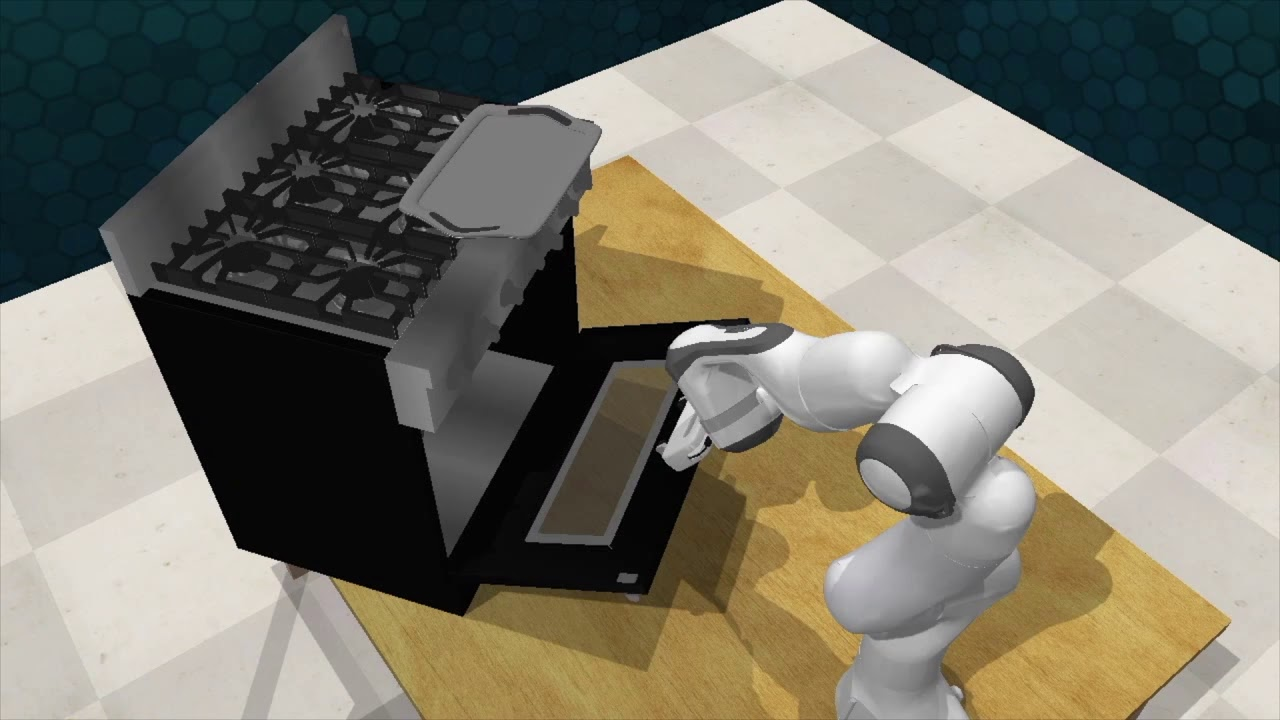
\includegraphics[width=\linewidth]{images/visual_control_envs/rl_bench.jpg}
    \end{subfigure}
    \caption{Различные среды визуального контроля}
    \end{figure}
\end{column}
\end{columns}

% \begin{minipage}[t]{0.48\linewidth}
%     Typical visual control environment:
%     \begin{itemize}
%         \item Directly controlled actuator
%         \item Success implies interaction between actuator and the object
%         \item OOD is extremely hard
%         % TODO: Replace by video...
%     \end{itemize}
%     \begin{figure}
%     \begin{subfigure}{.49\textwidth}
%         \centering
%             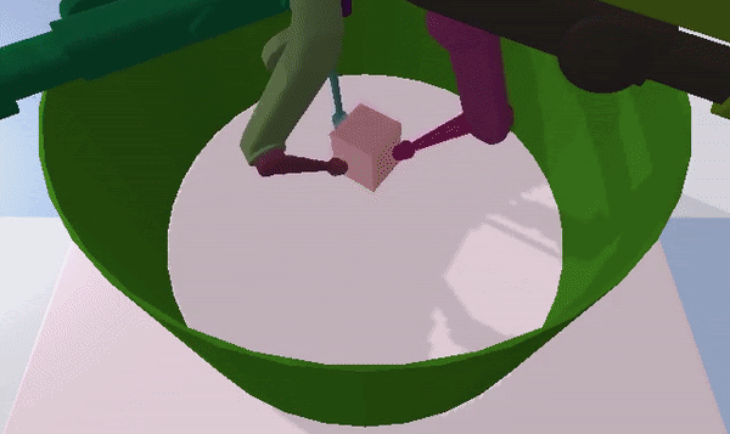
\includegraphics[width=0.9\linewidth]{images/visual_control_envs/causal_world.png}
%     \end{subfigure}
%     \begin{subfigure}{.49\textwidth}
%         \centering
%             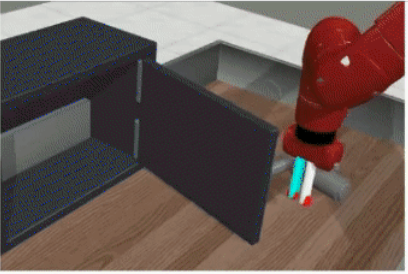
\includegraphics[width=0.9\linewidth]{images/visual_control_envs/metaworld.png}
%     \end{subfigure}
%     \end{figure}
% \end{minipage}
% \hfill
% \begin{minipage}[t]{0.48\linewidth}
%     \begin{figure}
%     \begin{subfigure}{.49\textwidth}
%         \centering
%           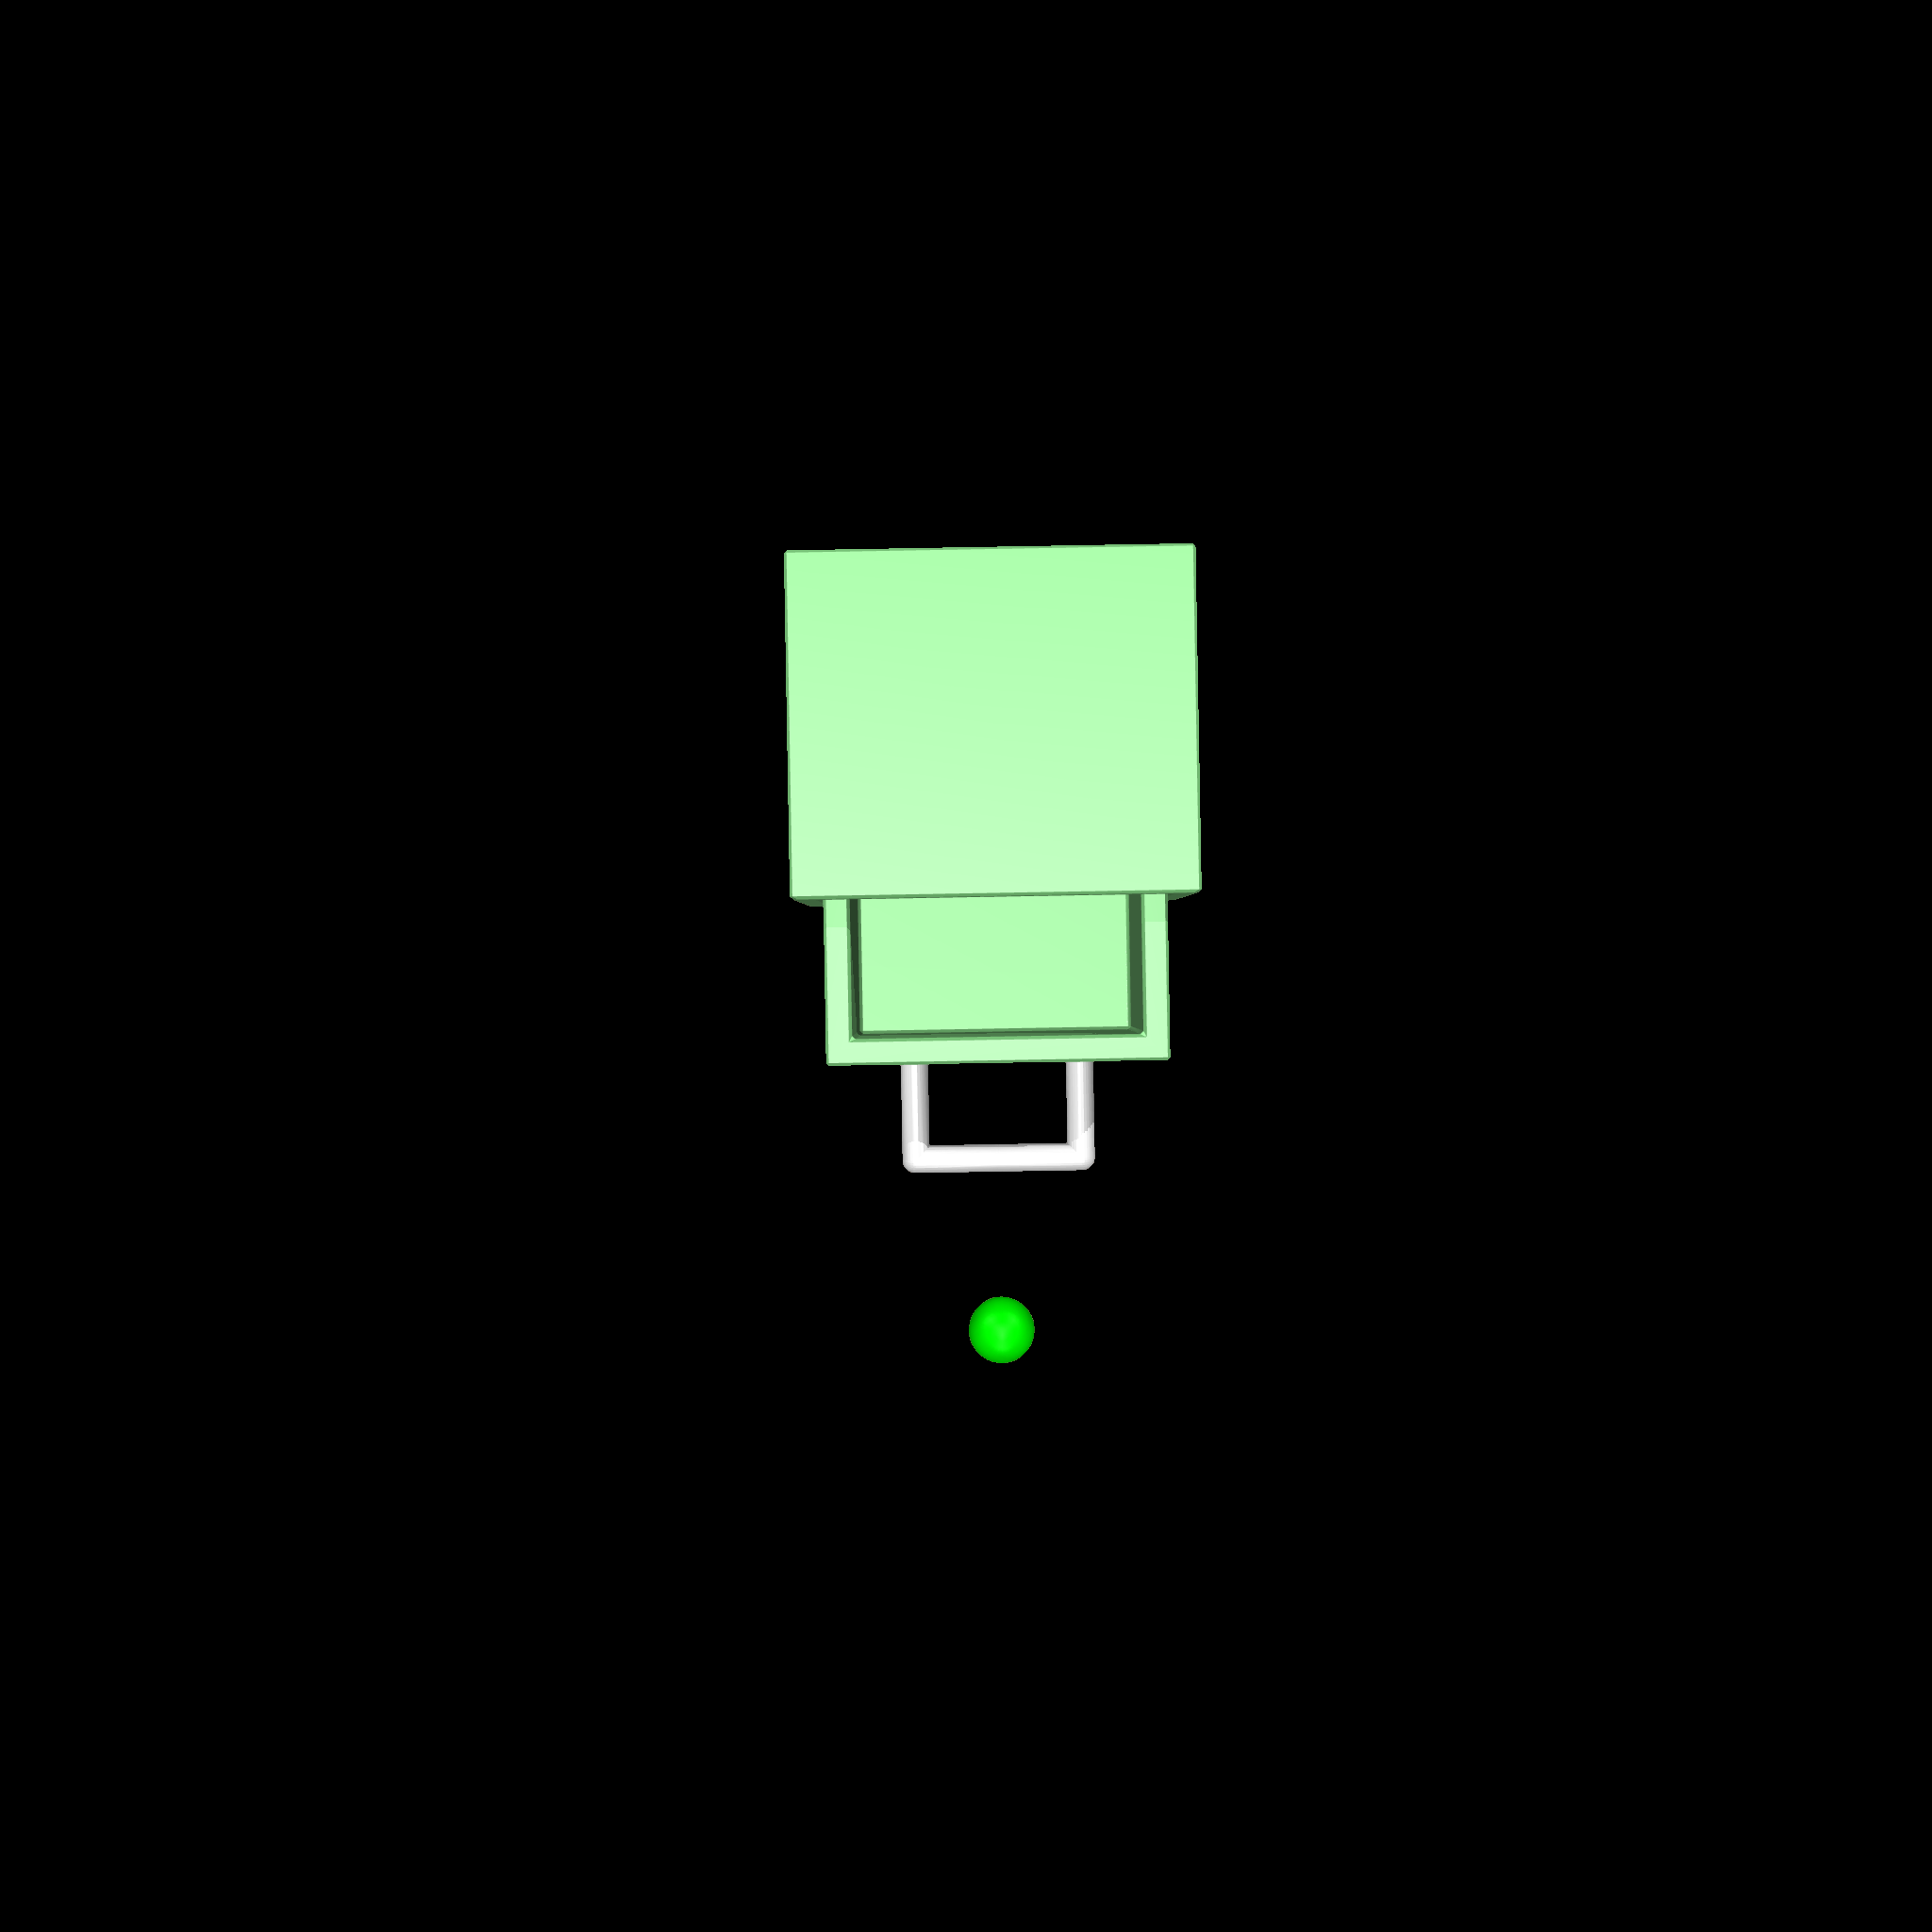
\includegraphics[width=0.9\linewidth]{images/env/masked_obj.png}
%     \end{subfigure}
%     \begin{subfigure}{.49\textwidth}
%         \centering
%           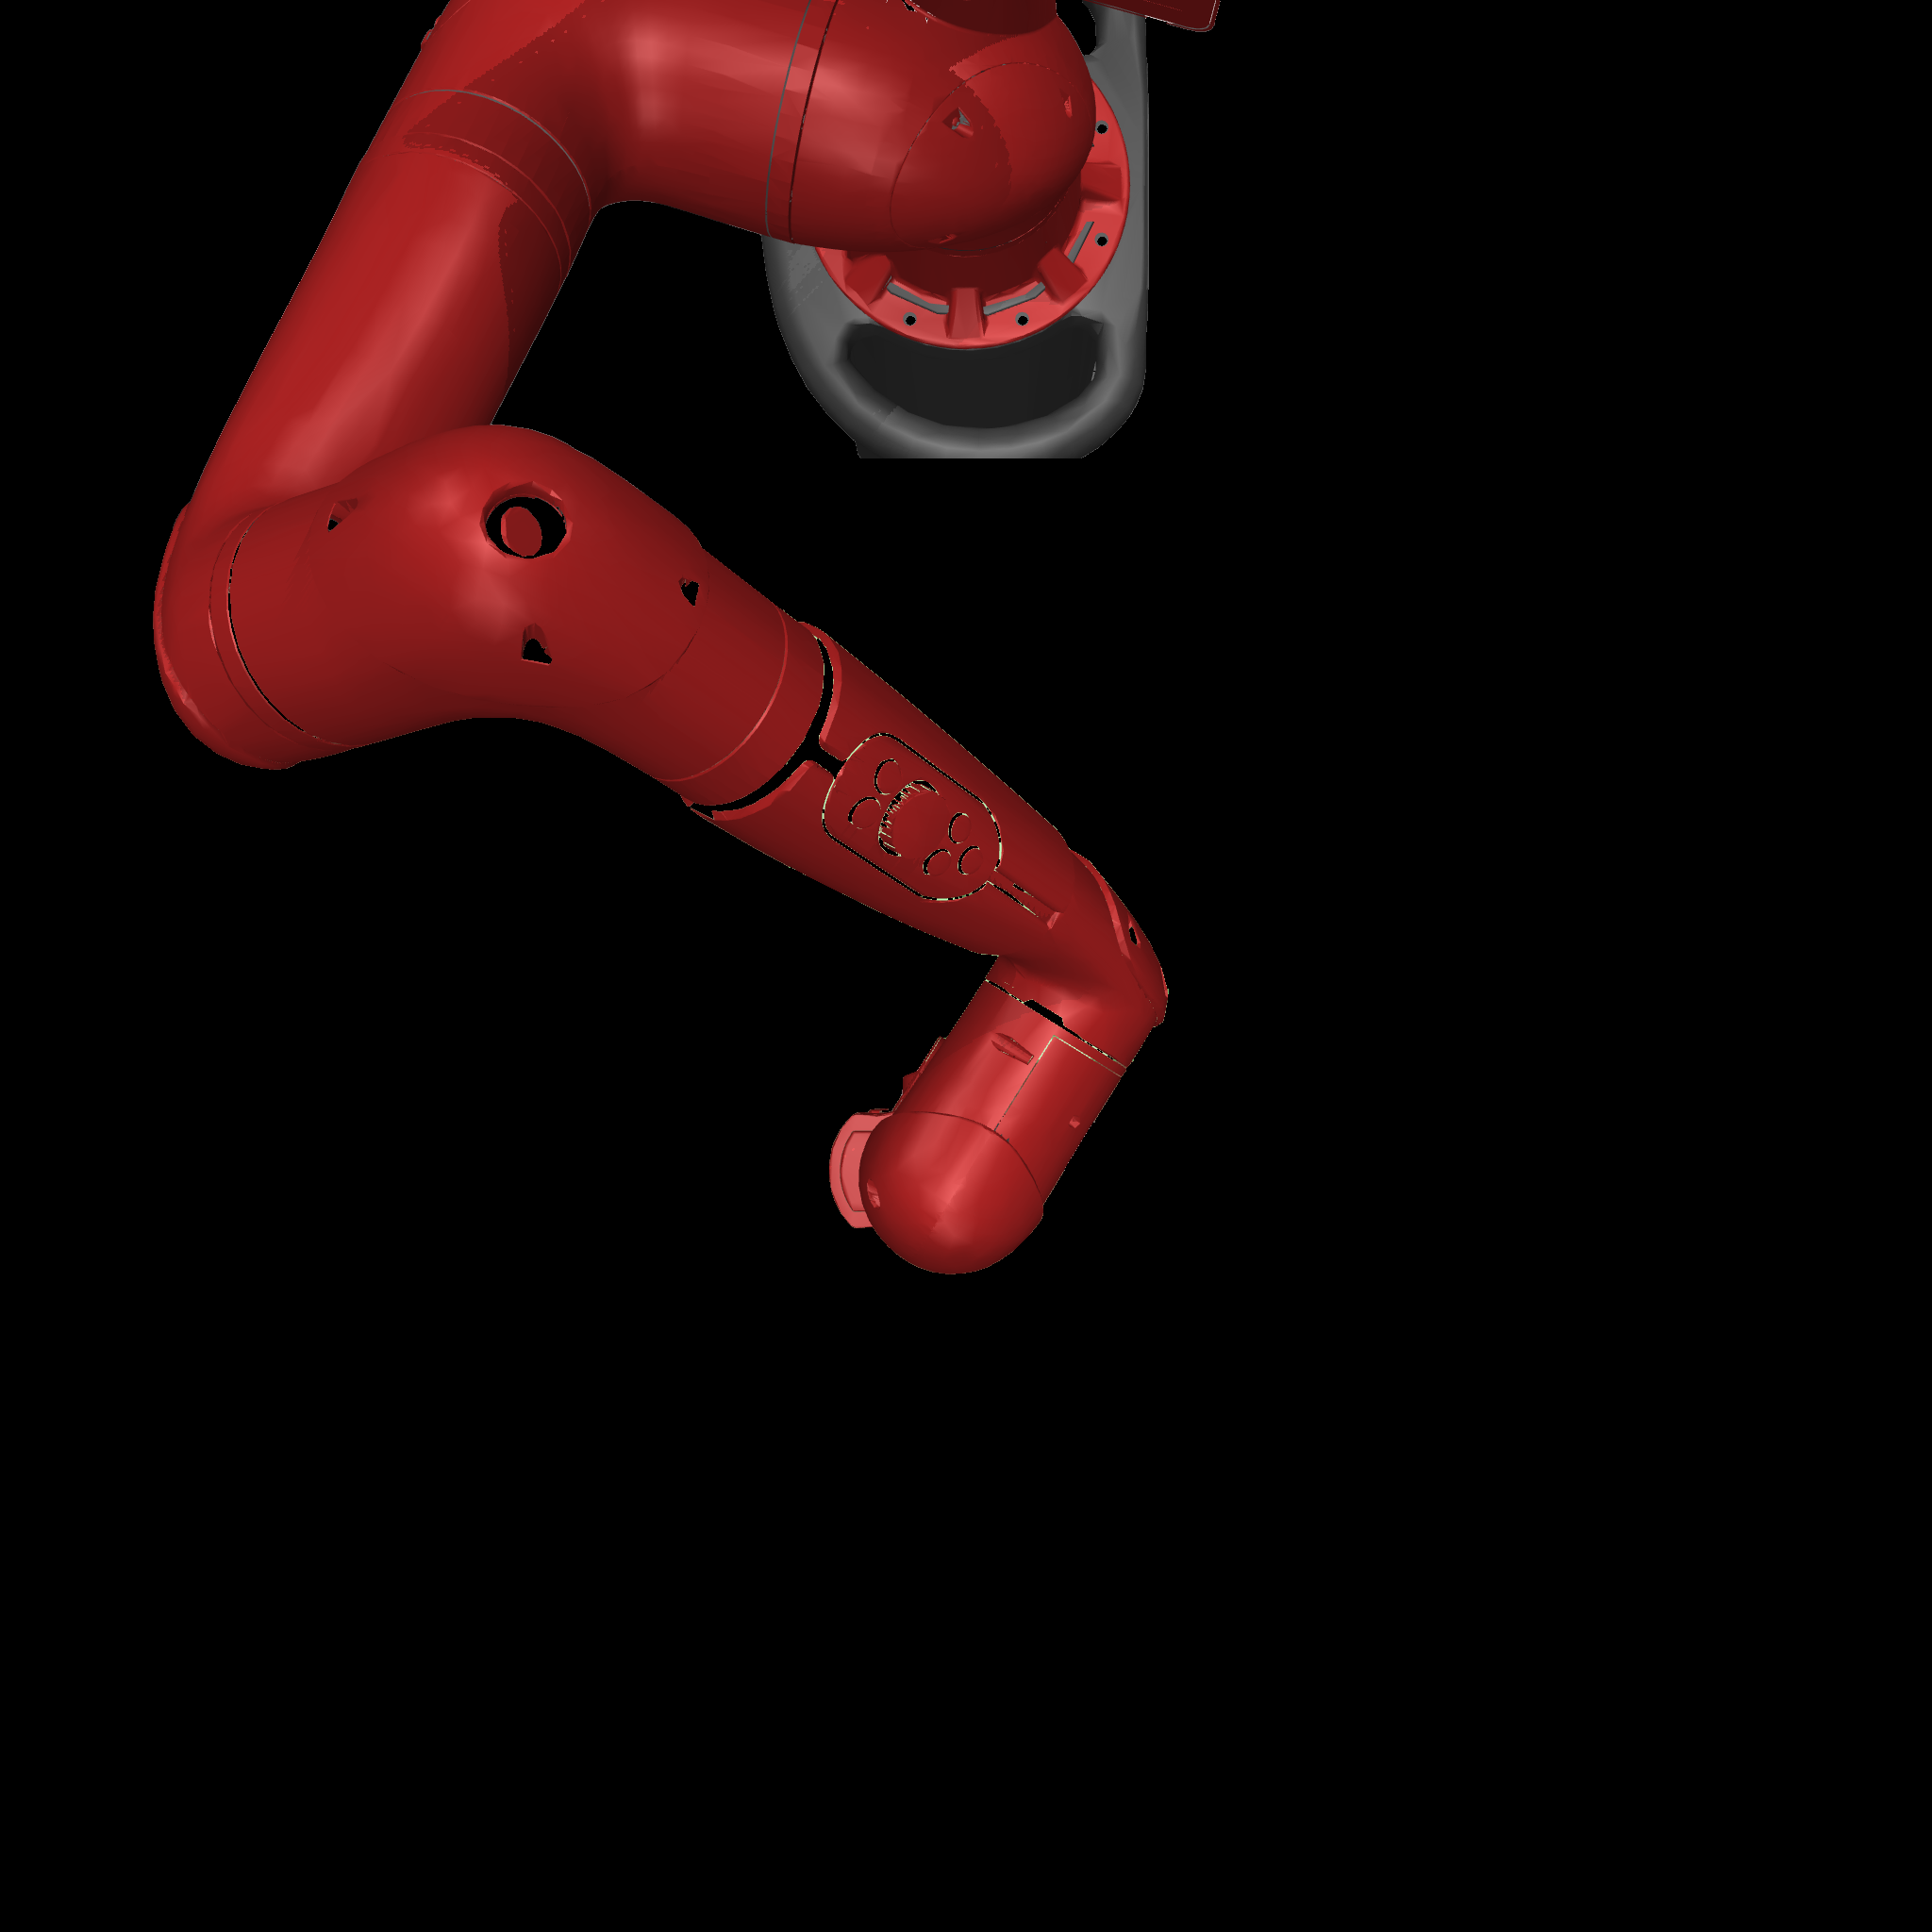
\includegraphics[width=0.9\linewidth]{images/env/masked_robot.png}
%     \end{subfigure}
%     \end{figure}
    
%     We can introduce structure:
%     \begin{itemize}
%         \item Each observation contains two entities of interest
%         \item Each entity have its own dynamics
%         \item Actor can directly affect or have a long-term influence over object
%     \end{itemize}
% \end{minipage}
\end{frame}

\note{
Many visual control tasks have the following features: there is a single directly controlled by actions manipulator, there is a number of objects, which can not be controlled by agent directly, and successful completion of task involves some type of interaction between actor and object, for example, opening the fridge. We introduce the object-oriented structure to World Model by factoring it.
}